\documentclass{article}
\usepackage{tikz}
\usetikzlibrary{angles, quotes}
\usepackage{amssymb}
\usepackage{pgfplots}
\pgfplotsset{width=10cm,compat=1.9}
\usepgfplotslibrary{statistics}
\usepackage[left=2.54cm,right=2.54cm,top=2.54cm,bottom=2.54cm]{geometry}
\usepackage{tasks} %Paquete necesario para la producción de items horizontales para algunos ejercicios de tarea empleando el comando /begin{multicols}}{#}.../end{multicols} para ayudarnos a reducir las páginas
\usepackage{pdflscape} %comando que permite cambiar a orientación horizontal las hojas%
\usepackage{soul} %Paquete para permitir la compilación de acentos usando el comando {\hl{}}}\\
\sethlcolor{yellow(munsell)} %comando para definir el color para el subrayado usando el comando \hl
\usepackage[utf8]{inputenc}
\usepackage[spanish]{babel}
\usepackage{icomma}
\usepackage{ragged2e}
\usepackage{siunitx}
\usepackage{url}
\usepackage[colorlinks=true, urlcolor=blue,  linkcolor=Cerulean, citecolor=green]{hyperref}
\usepackage{pdfpages}
\usepackage{blindtext} %Paquete que genera texto ficticio (dummy text) con el comando: \blindtext
\usepackage{cancel} %in the preamble gives you four different modes of striking through: \cancel{text to cancel} draws a diagonal line (slash) through its argument, \bcancel{text to cancel} uses the negative slope (a backslash), \xcancel{text to cancel} draws an X (actually \cancel plus \bcancel), \cancelto{〈value〉}{〈expression〉} draws a diagonal arrow through the 〈expression〉pointing to the 〈value〉 (math-mode only)
\usepackage{csquotes}
\usepackage{afterpage}
\usepackage{parskip} 
\usepackage{float}
\usepackage{enumitem}
\usepackage{multicol}%Paquete que permite la creación aislada de columnas de texto. De esta forma se reduce la cantidad de páginas en nuestro documento
\usepackage{lipsum} %Paquete que genera texto de relleno al igual que \usepackage{blindtext}, se usa con el comando \lipsum[#-#] los #(hashtags) delimitan el número de páginas que deseamos ocupar del paquete lipsum para usarlos como relleno. 

% Definir el comando personalizado para la nota
\newcommand{\mynote}[1]{%
\begin{tikzpicture}[baseline=-0.75ex]
	\node[draw, circle, fill=Apple Green!60, inner sep=2pt] (note) {\textbf{Nota:}};
\end{tikzpicture}%
\ \textit{#1}%
}

\newenvironment{Figura}
{\par\medskip\noindent\minipage{\linewidth}}
{\endminipage\par\medskip}
\usepackage{caption}
\usepackage[
backend=biber,
sorting=none,
url=true
]{biblatex} %bibliografía
\addbibresource{biblio.bib}
% Establecer el espacio entre las entradas de la bibliografía
\setlength{\bibitemsep}{1\baselineskip} % Puedes ajustar el valor según tus preferencias
\usepackage{amsmath,amsthm,amssymb,amsfonts}
\usepackage{pifont} %Permite la compilación del comando \xmark: es el símbolo de la tachita
\usepackage{mathtools} %permite la compilación de símbolos para matrices
\usepackage{empheq} %Paquete que se relaciona con \usepackage[most]{tcolorbox} para la creación de cuadros/cajas de colores para delimitar los resultados matemáticos o líneas de texto usando la línea de comando: \begin{empheq}[box={\mymath[colback=orange(webcolor)!70,drop lifted shadow]}]{equation*} \end{empheq}
\usepackage[most]{tcolorbox} %Paquete que se relaciona con \usepackage{empheq} para la creación de cuadros/cajas de colores para delimitar los resultados matemáticos o líneas de texto
\renewcommand{\qedsymbol}{$\blacksquare$}
\usetikzlibrary{positioning,decorations.pathreplacing} %Paquete que permite la compilación de llaves para cuadros sinópticos (brace diagram) 
\usepackage{schemata} %The schemata package is designed just for these brace diagrams
\usepackage{booktabs}

\newcommand\AB[2]{\schema{\schemabox{#1}}{\schemabox{#2}}} %comando o paquete necesario para crear cuadros sinópticos

\newtcbox{\mymath}[1][]{%
nobeforeafter, math upper, tcbox raise base,
enhanced, colframe=blue!30!black,
colback=blue!30, boxrule=1pt,
#1} %Comando importante para encasillar los resultados matemáticos en cajas de diferentes colores, se relaciona con los paquetes \usepackage{empheq} y \usepackage[most]{tcolorbox} 

\newenvironment{sysmatrix}[1]
{\left(\begin{array}{@{}#1@{}}}
{\end{array}\right)}
\newcommand{\ro}[1]{%
\xrightarrow{\mathmakebox[\rowidth]{#1}}%
}
\newlength{\rowidth}% row operation width
\AtBeginDocument{\setlength{\rowidth}{3em}}  %Comando importante para laproducción de lineas de operaciones entre matrices, método de Gauss o Gauss Jordan se relaciona con \newenvironment{sysmatrix}

%formato para cambiar el horario a español
\usepackage[spanish]{datetime2}
\DTMsetdatestyle{spanish}

\renewcommand{\today}{\DTMdisplaydate{\the\year}{\the\month}{\the\day }{-1}}
%%%%%%%%%%%%%%%%%%%%%%%%%%%%%%%%%%%%%%%%%

\usepackage{datetime}
\newcommand{\mycurrenttime}{\xxivtime}

%%%%%%%%%%%%%%%%%%%%%%%%%%%%%%%%%%%%%%%%%%%%%%%%%%%%%%%%%%%%%%%%%%%%%%%%%%%%%%%%%%%%%%%%%%%%%%%%%%%%%%%%%%%%%%%%%%%%%%%%%%%%%%%%%%%%%%%%%%%%%%%%%


%%%%%%%%%%%%%Caja de color para el título%%%%%%%%%%%%%%%%%%%%%%%%%%%%%%%%%%%%%%%%%%%%%%%%%%%%%%

\definecolor{myframecolor}{RGB}{1, 45, 75} % Prussian Blue
\definecolor{myboxcolor}{RGB}{0, 107, 92} % Apple Green

\newtcolorbox{mybox}{
enhanced,
colback=myboxcolor!7, % Color de fondo del cuadro
colframe=myframecolor, % Color del marco del cuadro
arc=0pt,
boxrule=1pt,
borderline west={2mm}{-10mm}{myframecolor}, % Borde en el lado izquierdo
sharp corners=southwest,
width=\linewidth,
before=\par\vspace{\bigskipamount}, % Espacio antes del cuadro
after=\par\vspace{\bigskipamount} % Espacio después del cuadro
}


\newcommand{\euler}{e} %Comando para producir letra e de euler
\newenvironment{remark}{\par\vfill\footnotesize % Vertical white space above the remark and smaller font size
\begin{list}{}{
		\leftmargin=80pt % Indentation on the left
		\rightmargin=60pt}\item\ignorespaces % Indentation on the right
	\makebox[-2.5pt]{\begin{tikzpicture}[overlay]
			\node[draw=Horizon!60,line width=2.5pt,circle,fill=Horizon!25,font=\sffamily\bfseries,inner sep=4pt,outer sep=0pt] at (-19pt,5pt){\textcolor{Horizon}{Nota}};\end{tikzpicture}} % Blue Nota in a circle
	\advance\baselineskip -1pt}{\end{list}\vskip5pt} % Tighter line spacing and white space after remark
	\usepackage{graphicx}
	
	\usepackage{titling}
	
	\input{colores.tex}
	
	%%Producir signos de cita textual``Asignatura''
	
	\newcommand{\xmark}{\ding{55}} %%%comando que genera la tachita
	
	\newenvironment{MyColorPar}[1]{%
\leavevmode\color{#1}\ignorespaces%
}{%
}%

%%%%%%%%%%%%%%%%%%% Título de la tarea, Nombre de alumno

\title{\textbf{Bitácora} (extracciones de café) - \textcolor{Apple Green}{\textbf{Colombia Gourmet}}, \textcolor{Tarawera}{\textbf{Colombia Selecto}}, \textcolor{Cinnabar}{\textbf{Pluma Hidalgo}}, \textcolor{Sun}{\textbf{Pahuatlán (Pue)}} }
\author{\emph{\textbf{CAFELAB}} $\boldsymbol{\mid}$}
\date{\today}

%%%%%%%%%%%%%%%%%%% Datos de la Materia

\usepackage{fancyhdr}
\fancypagestyle{plain}{%  the preset of fancyhdr 
\fancyhf{} % clear all header and footer fields
\fancyfoot[R]{
\includegraphics[width=2cm]{LogoFCFMBUAP (1).png}}
\fancyfoot[L]{{\bfseries{\thedate{}}} a las {\bfseries{\mycurrenttime{}}} horas{} (GMT-6, H. Puebla de Zaragoza, Pue)}
\fancyhead[L]{Laboratorio de caracterización de materiales}
\fancyhead[R]{\theauthor}
}
\makeatletter
\def\@maketitle{%
\newpage
\null
\vskip 1em%
\begin{center}%
	\let \footnote \thanks
	{\LARGE \@title \par}%
	\vskip 1em%
	%{\large \@date}%
\end{center}%
\par
\vskip 1em}
\makeatother

\usepackage{lipsum}  
\usepackage{cmbright}


%%%%%%%%%%%%%%%%%%%%%%%%%%%%%%%%%%%%%%%%%%%%%%%%%%%%%%%%%%%%%%%%%%%%%%%%%%%%%%%%%%%%%%%%%%%%%%%%%%%%%%%%%%%%%%%%%%%%%%%%%%%%%%%%%%%%%%%%%%%%%%%%%%%%%%%%%%%%%%%%%%%%%%%%%%%%%%%%%%%%%%%%%%%%%%%%%%%%%%

\begin{document}



\maketitle


%%%%%%%%%%%%%%%%%%% Datos del profesor, campus y aula

\begin{mybox}
  \noindent\begin{tabular}{@{}ll}
    {\bfseries{Profesor}} & Dr. Martín Rodolfo Palomino Merino\\
    \textcolor{prussianblue}{\bfseries{Campus}} / \textcolor{trueblue}{\bfseries{Facultad}}  & \textcolor{prussianblue}{\bfseries{C.U. BUAP}} /  \textcolor{trueblue}{\bfseries{FCFM}} \\
    \textcolor{prussianblue}{\bfseries{Edificio}} /  \textcolor{trueblue}{\bfseries{Salón}}    &   \textcolor{prussianblue}{\bfseries{1FM1}} /  \textcolor{trueblue}{\bfseries{301}} \\
    \textcolor{prussianblue}{\bfseries{Integrante}} & \textbf{Lizeth Jampin Orozco García} \\
    \textcolor{prussianblue}{\bfseries{Integrante}} & \textbf{Julio Alfredo Ballinas García} \\
    \textcolor{prussianblue}{\bfseries{Colaborador}} & \textbf{Roberto Álvarez Zavala}
  \end{tabular}
\end{mybox}\vspace{1cm}





\vspace{2cm}
% Solo el TOC en negro
\hypersetup{linkcolor=black}
\tableofcontents
% Restaura Cerulean para el resto del documento
\hypersetup{linkcolor=Cerulean}
 \vspace{2cm}

\section{Nuevo café: Pluma Hidalgo (Oaxaca)}

Tenemos una nueva muestra de café (\textbf{fecha: 08/10/2025}), está café fue entregado por el Dr. Martín Rodolfo Palomino, el cual por medio de \emph{Blanca Azucena} se obtuvo un café de Oaxaca llamado \underline{Pluma Hidalgo}.

\section{Pastilas para \textcolor{orange(colorwheel)}{\textbf{reflectancia}} y \textcolor{Cerulean}{\textbf{fluorescencia}}}

Ya se tienen las pastillas para \textcolor{orange(colorwheel)}{\textbf{reflectancia}}  y \textcolor{Cerulean}{\textbf{fluorescencia}}  siguientes: 

\begin{itemize}
\item[$\bullet$]
\[
\textbf{Chiapas}
\left\{
\begin{array}{cc}
\textcolor{Cerulean}{\textbf{Fluorescencia}} \to \textbf{tag: }(xCh) & \left\{\begin{array}{c}\text{Se tienen 2 pastillas}\end{array}\right.\\
\textcolor{orange(colorwheel)}{\textbf{Reflectancia}} \to \textbf{tag: }(RCh) & \left\{\begin{array}{c}\text{Se tienen 2 pastillas}\end{array}\right.
\end{array}
\right.
\]

\item[$\bullet$]
\[
\textbf{Guerrero}
\left\{
\begin{array}{cc}
\textcolor{Cerulean}{\textbf{Fluorescencia}} \to \textbf{tag: }(xGo) & \left\{\begin{array}{c}\text{Se tienen 2 pastillas}\end{array}\right.\\
\textcolor{orange(colorwheel)}{\textbf{Reflectancia}} \to \textbf{tag: }(RGo) & \left\{\begin{array}{c}\text{Se tienen 2 pastillas}\end{array}\right.
\end{array}
\right.
\]

\item[$\bullet$]
\[
\textbf{Oaxaca}
\left\{
\begin{array}{cc}
\textcolor{Cerulean}{\textbf{Fluorescencia}} \to \textbf{tag: }(xOx) & \left\{\begin{array}{c}\text{Se tienen 2 pastillas}\end{array}\right.\\
\textcolor{orange(colorwheel)}{\textbf{Reflectancia}} \to \textbf{tag: }(ROx) & \left\{\begin{array}{c}\text{Se tienen 2 pastillas}\end{array}\right.
\end{array}
\right.
\]

\item[$\bullet$]
\[
\textbf{Veracruz}
\left\{
\begin{array}{cc}
\textcolor{Cerulean}{\textbf{Fluorescencia}} \to \textbf{tag: }(xVe) & \left\{\begin{array}{c}\text{Se tienen 2 pastillas}\end{array}\right.\\
\textcolor{orange(colorwheel)}{\textbf{Reflectancia}} \to \textbf{tag: }(RVe) & \left\{\begin{array}{c}\text{Se tienen 2 pastillas}\end{array}\right.
\end{array}
\right.
\]

\item[$\bullet$]
\[
\textbf{Mixteca Alta Oaxaqueña}
\left\{
\begin{array}{cc}
\textcolor{Cerulean}{\textbf{Fluorescencia}} \to \textbf{tag: }(xMi) & \left\{\begin{array}{c}\text{Se tienen 2 pastillas}\end{array}\right.\\
\textcolor{orange(colorwheel)}{\textbf{Reflectancia}} \to \textbf{tag: }(RMi) & \left\{\begin{array}{c}\text{Se tienen 2 pastillas}\end{array}\right.
\end{array}
\right.
\]

\item[$\bullet$]
\[
\textbf{Puebla (Pahuatlán)}
\left\{
\begin{array}{cc}
\textcolor{Cerulean}{\textbf{Fluorescencia}} \to \textbf{tag: }(xPu) & \left\{\begin{array}{c}\text{Se tienen 2 pastillas}\end{array}\right.\\
\textcolor{orange(colorwheel)}{\textbf{Reflectancia}} \to \textbf{tag: }(RPu) & \left\{\begin{array}{c}\text{Se tienen 2 pastillas}\end{array}\right.
\end{array}
\right.
\]

\item[$\bullet$]
\[
\textbf{Colombia (Gourmet)}
\left\{
\begin{array}{cc}
\textcolor{Cerulean}{\textbf{Fluorescencia}} \to \textbf{tag: }(CoG \, y \,  xCoG ) & \left\{\begin{array}{c}\text{Se tienen 2 pastillas}\end{array}\right.\\
\textcolor{orange(colorwheel)}{\textbf{Reflectancia}} \to \textbf{tag: }(RCoG) & \left\{\begin{array}{c}\text{Se tienen 2 pastillas}\end{array}\right.
\end{array}
\right.
\]

\item[$\bullet$]
\[
\textbf{Colombia (Selecto)}
\left\{
\begin{array}{cc}
\textcolor{Cerulean}{\textbf{Fluorescencia}} \to \textbf{tag: }(CoS\, y\, CoS) & \left\{\begin{array}{c}\text{Se tienen 2 pastillas}\end{array}\right.\\
\textcolor{orange(colorwheel)}{\textbf{Reflectancia}} \to \textbf{tag: }(RCoS) & \left\{\begin{array}{c}\text{Se tienen 2 pastillas}\end{array}\right.
\end{array}
\right.
\]

\item[$\bullet$]
\[
\textbf{Pluma Hidalgo (Oaxaca)}
\left\{
\begin{array}{cc}
\textcolor{Cerulean}{\textbf{Fluorescencia}} \to \textbf{tag: }(xPh) & \left\{\begin{array}{c}\text{Se tienen 2 pastillas}\end{array}\right.\\
\textcolor{orange(colorwheel)}{\textbf{Reflectancia}} \to \textbf{tag: }(RPh) & \left\{\begin{array}{c}\text{Se tienen 2 pastillas}\end{array}\right.
\end{array}
\right.
\]

\item[$\bullet$]
\[
\textbf{Illy}
\left\{
\begin{array}{cc}
\textcolor{Cerulean}{\textbf{Fluorescencia}} \to \textbf{tag: }(xIlly) & \left\{\begin{array}{c}\text{Se tienen 2 pastillas}\end{array}\right.\\
\textcolor{orange(colorwheel)}{\textbf{Reflectancia}} \to \textbf{tag: }(RIlly) & \left\{\begin{array}{c}\text{Se tienen 2 pastillas}\end{array}\right.
\end{array}
\right.
\]

\item[$\bullet$]
\[
\textbf{Cafeína}
\left\{
\begin{array}{cc}
\textcolor{Cerulean}{\textbf{Fluorescencia}} \to \textbf{tag: }(xCafeina) & \left\{\begin{array}{c}\text{Se tienen 2 pastillas}\end{array}\right.\\
\textcolor{orange(colorwheel)}{\textbf{Reflectancia}} \to \textbf{tag: }(RCafeina) & \left\{\begin{array}{c}\text{Se tienen 2 pastillas}\end{array}\right.
\end{array}
\right.
\]

\item[$\bullet$]
\[
\textbf{Verde}
\left\{
\begin{array}{cc}
\textcolor{Cerulean}{\textbf{Fluorescencia}} \to \textbf{tag: }(xVerde) & \left\{\begin{array}{c}\text{Se tienen 2 pastillas}\end{array}\right.\\
\textcolor{orange(colorwheel)}{\textbf{Reflectancia}} \to \textbf{tag: }(RVerde) & \left\{\begin{array}{c}\text{Se tienen 2 pastillas}\end{array}\right.
\end{array}
\right.
\]

\item[$\bullet$]
\[
\textbf{Mucilago}
\left\{
\begin{array}{cc}
\textcolor{Cerulean}{\textbf{Fluorescencia}} \to \textbf{tag: }(xMucilago) & \left\{\begin{array}{c}\text{Se tienen 2 pastillas}\end{array}\right.\\
\textcolor{orange(colorwheel)}{\textbf{Reflectancia}} \to \textbf{tag: }(RMucilago) & \left\{\begin{array}{c}\text{Se tienen 2 pastillas}\end{array}\right.
\end{array}
\right.
\]
\end{itemize}

Ya tenemos UV/Vis en gramajes (\textbf{7.5 g}, \textbf{15 g}, \textbf{18 g}, \textbf{22.5 g}) de las siguientes muestras:

\begin{itemize}
\item[$\star$] Oaxaca \textcolor{Apple Green}{\textbf{\checkmark \checkmark}}
\item[$\star$] Veracruz \textcolor{Apple Green}{\textbf{\checkmark \checkmark}}
\item[$\star$] Chiapas \textcolor{Apple Green}{\textbf{\checkmark \checkmark}}
\item[$\star$] Mixteca Alta Oaxaqueña \textcolor{Apple Green}{\textbf{\checkmark \checkmark}}
\item[$\star$] Illy (hace falta en \textbf{7.5 g}, \textbf{18 g}, \textbf{22.5 g}) \textcolor{Apple Green}{\textbf{\checkmark \checkmark}}
\item[$\star$] Guerrero \textcolor{Apple Green}{\textbf{\checkmark \checkmark}}
\item[$\star$] Puebla (Pahuatlán) \textcolor{Apple Green}{\textbf{\checkmark \checkmark}}
\item[$\star$] Pluma Hidalgo (\textbf{revisar los datos de \textcolor{Cinnabar}{\textbf{transmitancia}}, dado que en el cuarzo se realizó con una sola gota en lugar de \textcolor{vividviolet}{\textbf{5}}}) \textcolor{Apple Green}{\textbf{\checkmark \checkmark}}
\item[$\star$] Colombia Selecto (faltan los gramajes de \textbf{7.5 g}, \textbf{18 g} y \textbf{22.5 g}; después de la lectura de este texto los datos ya se encuentran recolectados) \textcolor{Apple Green}{\textbf{\checkmark \checkmark}}
\item[$\star$] Colombia Gourmet (faltan los gramajes de \textbf{7.5 g}, \textbf{18 g} y \textbf{22.5 g}) \textcolor{Apple Green}{\textbf{\checkmark \checkmark}}
\item[$\star$] Hace falta el \underline{café de especialidad} en todos los gramajes (adquirido por \textbf{Lizeth} en \emph{Espíritu Café})
\end{itemize}


\section{Extracción Pluma Hidalgo}

Extraemos 15 gramos de \underline{Pluma Hidalgo} en la \textbf{prensa francesa} (luego llevamosa  espectro para UV-/Vis en \underline{Abs} y \underline{Trans}).

\begin{itemize}
\item[$\bullet$] \textbf{Nota:} La molienda es bastante fina, posiblemente el perfil de sabor sea \underline{amargo} (debido a la molienda, en prensa francesa la molienda debe de ser un poco más gruesa)
\end{itemize}

\subsection{Pesos aproximados en la balanza}

\begin{itemize}
\item[$\bullet$] \textbf{7.5\,g}\\
\textit{Peso aproximado} = 7.506\,g\\
\item[$\bullet$] \textbf{15\,}\\
\textit{Peso aproximado} = 15.0192\,g\\
\item[$\bullet$] \textbf{18\,g}\\
\textit{Peso aproximado} = 18.0049g\,g \\
\item[$\bullet$] \textbf{22.5\,g}\\
\textit{Peso aproximado} = 22.5\,g
\end{itemize}


\section{Ecuación de concentración masa - volumen}

Sucede que cada vez tenemos menos \underline{café molido} para \textbf{Colombia} (S) y (G), entonces es complicado reproducir las mediciones de:

\begin{itemize}
\item[$\bullet$] 7.5 g
\item[$\bullet$] 15 g
\item[$\bullet$] 18 g
\item[$\bullet$] 22.5 g
\end{itemize}

dado que la cantidad de café disponible es poca y no alcanza para las tareas de mediciones en el espectrómetro, nos vemos en la necesidad de trabajar con la siguiente ecuación de concentración:

\subsection{Ejemplo práctico para 18\,g}

\begin{equation}
\begin{split}
C &= \frac{m}{v}
\end{split}
\end{equation}

Donde:

\begin{itemize}
\item[$\bullet$] $C = \text{concentración}$\\
\item[$\bullet$] $m = \text{masa}$\\
\item[$\bullet$] $v = \text{volumen}$
\end{itemize}

\underline{Por ejemplo}. Si nosotros tenemos $18g$ en $200ml$ como objetivo, entonces tenemos la siguiente concentración:

\begin{equation}
\begin{split}
 C_{1} &= \frac{18g}{200ml} = 0\text{.}09 \frac{g}{ml}
\end{split}\label{eq:2}
\end{equation}

\subsection{Brew ratio (relación café: agua)}

El \underline{inverso} la ecuación \ref{eq:2} nos da la razón \textcolor{Pesto}{\textbf{café}}: \textcolor{Cerulean}{\textbf{agua}} (brew ratio o relación de extracción), es decir:

\[ \left(C_{1}\right)^{-1} = \frac{  200ml }{ 18g } = \frac{1}{0\text{.}09} = 11\text{.}1 \frac{ml}{g}  \]

La proporción es:

\[\boxed{1:11\text{.}1}, \quad \text{es decir 1 g de café por cada 11 ml de agua}\]

(En términos de café filtrado es una \underline{relación concentrada})

La de prensa francesa va de $\boxed{1:13} - \boxed{1:20}$. 

\subsection{Caso en donde tengamos poco café}

Si tenemos poco café lo que buscamos es que se extraiga la misma concentración, es decir; originalmente tenemos un \textbf{ratio} o \textbf{concentración} de $x$ cantidad, entonces con cierta cantidad de soluto vamos a repoducir la misma \textbf{concentración} o \textbf{ratio}.  Tenemos:

\[ C_{1} = C_{2} \]

Donde: 

\begin{itemize}
\item[$\star$] $C_{1}$. Es la concentración inicial.\\
\item[$\star$] $C_{1}$. Es la concentración final.
\end{itemize}

Tenemos para un caso en donde tengamos sólo $5g$ de café.

\begin{equation}
\begin{split}
 \frac{m_{1}}{v_{1}} &= \frac{ m_{2} }{v_{2}}
\end{split} \label{eq:3}
\end{equation}

De donde: 

\begin{itemize}
\item[$\bullet$] $m_{1} = 18g$\\
\item[$\bullet$] $v_{1} = 200ml$\\
\item[$\bullet$] $m_{2} = 5g$\\
\item[$\bullet$] $v_{2} = ?$\\
\end{itemize}

Haciendo un despeje para $V_{2}$ tenemos:

\begin{equation}
\begin{split}
    v_{2} &= \left( \frac{ m_{2} }{m_{1}}  \right) \cdot v_{1} \quad \Rightarrow \quad v_{2} = \left( \frac{5g}{18g} \right) \cdot (200ml)  = 55\text{.}6ml
\end{split} 
\end{equation}

Es decir, se necesitan $55\text{.}6\,ml$ de agua para mantener la misma concentración inicial. \emph{Esto mantiene la misma intensidad de extracción sin que la bebida quede más diluida o concentrada}

\section{Extracción Café Colombia selecto}

Para este café ya tenemos los datos en el gramaje de 15\,g, ahora necesitamos reproducir los demás gramajes.

Tenemos 28.92\,g totales de café \textbf{Colombia (selecto)} y es necesario extraer en \textbf{7.5\,g}, \textbf{18\,g} y \textbf{22.5\,g}. Vamos a ocupar la ecuación \ref{eq:3} para calcular los volumenes necesarios para mantener la concentración inicial ($C_{1}$)9, ocuparíamos un total de $\mathbf{9\text{.}64g}$ por muestra (gramaje). 

\subsection{Empleo de la ecuación de concentración masa -  volumen (no hay suficiente café)}

Tenemos $\ldots$

\begin{itemize}
\item[$\bullet$] \textbf{7.5g} \\
Peso aproximado en la balanza $\approx$  9.64 $g$.\\
Empleando la ecuación \ref{eq:3} tenemos el siguiente volúmen necesario:
\[  v_{2} = \left(  \frac{9\text{.}64g   }{7\text{.}5g}  \right) 200\, ml = 257\text{.}07\, ml  \]
\textbf{Verificación}
\begin{equation*}
\begin{split}
 \frac{m_{1}}{v_{1}} = \frac{ m_{2} }{v_{2}} \quad \to \quad \frac{ 7\text{.}5\, g  }{200 \, ml} &= \frac{ 9\text{.}64\, g }{257\text{.}07\,ml}\\
0\text{.}0375 \frac{g}{ml} &= 0\text{.}03749 \frac{g}{ml} \\
\underbrace{\textbf{ratio}}_{\substack{\text{Inverso de la}\\\text{concentración (ec. \ref{eq:3})} \hspace{1mm} \underbrace{C}_{ \frac{m_{1}}{v_{1}} = \frac{m_{2}}{v_{2}} } \\ \text{Nos da la relación} \\ \text{de \textcolor{Pesto}{\textbf{café}}: \textcolor{Cerulean}{\textbf{agua}}} }}  \Rightarrow \quad  26\text{.}6 \frac{ml}{g} \,  \text{es decir} \, \boxed{\textcolor{Pesto}{\mathbf{1}}:\textcolor{Cerulean}{\mathbf{26\text{.}6}}}  & =  \boxed{1:26\text{.}66}
\end{split}
\end{equation*}
\end{itemize}

\begin{itemize}
\item[$\bullet$] \textbf{18g} \\
Peso aproximado en la balanza $\approx$  9.61 $g$.\\
Empleando la ecuación \ref{eq:3} tenemos el siguiente volúmen necesario:
\[  v_{2} = \left(  \frac{9\text{.}64g   }{18g}  \right) 200\, ml = 107\text{.}1\, ml  \]
\textbf{Verificación}
\begin{equation*}
\begin{split}
 \frac{m_{1}}{v_{1}} = \frac{ m_{2} }{v_{2}} \quad \to \quad \frac{ 18\, g  }{200 \, ml} &= \frac{ 9\text{.}64\, g }{107\text{.}1\,ml}\\
0\text{.}09 \frac{g}{ml} &= 0\text{.}090 \frac{g}{ml}\\
\textbf{ratio} \quad \Rightarrow \quad  \boxed{1:11\text{.}1} &= \boxed{1:11\text{.}1} 
\end{split}
\end{equation*}
\end{itemize}

\begin{itemize}
\item[$\bullet$] \textbf{22.5g} \\
Peso aproximado en la balanza $\approx$  9.644 $g$.\\
Empleando la ecuación de concentración  (ec.\ref{eq:3}) tenemos el siguiente volúmen necesario:
\[  v_{2} = \left(  \frac{9\text{.}64g   }{22\text{.}5g}  \right) 200\, ml = 85\text{.}68\, ml  \]
\textbf{Verificación}
\begin{equation*}
\begin{split}
 \frac{m_{1}}{v_{1}} = \frac{ m_{2} }{v_{2}} \quad \to \quad \frac{ 22\text{.}5\, g  }{200 \, ml} &= \frac{9\text{.}64\, g }{85\text{.}68\,ml}\\
0\text{.}1125 \frac{g}{ml} &= 0\text{.}112 \frac{g}{ml}\\
\textbf{ratio} \quad \Rightarrow \quad  \boxed{1:8\text{.}8} &= \boxed{1:8\text{.}8} 
\end{split}
\end{equation*}
\end{itemize}

\section{Extracción Café de Pahuatlán (Puebla)}

Necesitamos en total \textbf{63\,g} de café para producir las muestras de \textbf{7.5\,g}, \textbf{18\,g}, \textbf{15\,g} y \textbf{22.5\,g}.

En total en el envase se tienen \textbf{89.87 g}, entonces sí es posible que salgan todos los gramajes anteriores sin necesidad de emplear la ecuación \ref{eq:3}. 

\subsection{Pesos aproximados en la balanza}

\begin{itemize}
\item[$\bullet$] 7.5\,g\\
\textit{Peso aproximado} = 7.4988\,g\\
\item[$\bullet$] 15 \, g\\
\textit{Peso aproximado} = 15.04\,g\\
\item[$\bullet$] 18 \, g\\
\textit{Peso aproximado} = 18.0083\,g\\
\item[$\bullet$] 22.5 \, g\\
\textit{Peso aproximado} = 22.50\,g
\end{itemize} 

\subsection{Extracción en prensa francesa}

Extraemos las muestras anteriores a un volumen de\textbf{ 200\,ml} de agua. Es decir:

\subsubsection{Ratios de cada gramaje}

\begin{enumerate}
\item \textit{Medimos el agua total a usar en los vasos de precipitado}.
\item \textit{Posteriormente calentamos el agua en la parrilla hasta que ebulla. \textbf{Nota:} Una regla básica para determinar la temperatura de ebullición de la región es que por cada 300 msnm la temperatura de ebullición disminuye un grado centígrado. Es decir aplicar: \[T_{eb}(^{\circ}C)\approx100 - \frac{h}{300}\] Nos da una aproximación empírica últil. $h$ es la altura de la región en metros.}
\end{enumerate}

\begin{itemize}
\item[$\bullet$] Extraemos en la prensa \fbox{7.5\, g} en 200 ml de agua. Obtenemos un \textbf{ratio} de $\to$ $\boxed{ 1:26\text{.}6 }$
\item[$\bullet$] Extraemos en la prensa \fbox{15\, g} en 200 ml de agua. Obtenemos un \textbf{ratio} de $\to$ $\boxed{ 1:13\text{.}3}$
\item[$\bullet$] Extraemos en la prensa \fbox{18\, g} en 200 ml de agua. Obtenemos un \textbf{ratio} de $\to$ $\boxed{ 1:11\text{.}1}$
\item[$\bullet$] Extraemos en la prensa \fbox{22.5\, g} en 200 ml de agua. Obtenemos un \textbf{ratio} de $\to$ $\boxed{ 1:8\text{.}8}$ 
\end{itemize}

\subsection{Pesos aproximados en la balanza}

\begin{itemize}
\item[$\bullet$] \textbf{7.5\,g}\\
\textit{Peso aproximado} = 7.4977\,g\\
\item[$\bullet$] \textbf{15\,}\\
\textit{Peso aproximado} = 15.04\,g\\
\item[$\bullet$] \textbf{18\,g}\\
\textit{Peso aproximado} = 18.0083g\,g \\
\item[$\bullet$] \textbf{22.5\,g}\\
\textit{Peso aproximado} = 22.5063\,g
\end{itemize}

\section{Extracción Colombia gourmet (G)}

\textbf{Fecha: 09/10/2025}

Para este caso también ya se tienen los datos de \textbf{15\,g}, sin embargo contamos con una cantidad de café en la que no es posible reproducir todos los gramajes sin cambios en el peso, por consiguiente se realiza el mismo análisis que se hizo con el \textbf{café de Colombia selecto}.

Pesamos la cantidad total de café disponible en la bolsa y dividimos ese total entre 3 (dado que se reproducen concentraciones de \textbf{7.5\,g}, \textbf{18\,g} y \textbf{22.5\,g}). 

Usamos la ecuación \ref{eq:3} para calcular el \underline{volumen} de agua necesario para extraer la misma \emph{concentración}, es decir:

\[  \boxed{ C_{1} = C_{2} } \]

El peso total de \textbf{Café Colombia gourmet} disponible fue de \fbox{36.4891\,g}, Usamos $1/3$ de ese peso para cada extracción. Tenemos una proporción de \fbox{12.16\,g} por extracción. 



\subsection{Empleo de la ecuación de concentración masa -  volumen (no hay suficiente café)}

Tenemos $\ldots$

\begin{itemize}
\item[$\bullet$] \textbf{7.5g} \\
Peso aproximado en la balanza \textit{no fue anotado, pero se verificó que estuviese cerca de 12.16 en la balanza}.\\
Empleando la ecuación \ref{eq:3} tenemos el siguiente volúmen necesario:
\[  v_{2} = \left(  \frac{12\text{.}16g   }{7\text{.}5g}  \right) 200\, ml = 324\text{.}26\, ml  \]
\textbf{Verificación}
\begin{equation*}
\begin{split}
 \frac{m_{1}}{v_{1}} = \frac{ m_{2} }{v_{2}} \quad \to \quad \frac{ 7\text{.}5\, g  }{200 \, ml} &= \frac{12\text{.}16\, g }{257\text{.}07\,ml}\\
0\text{.}0375 \frac{g}{ml} &= 0\text{.}0375 \frac{g}{ml} \\
\underbrace{\textbf{ratio}}_{\substack{\text{Inverso de la}\\\text{concentración (ec. \ref{eq:3})} \hspace{1mm} \underbrace{C}_{ \frac{m_{1}}{v_{1}} = \frac{m_{2}}{v_{2}} } \\ \text{Nos da la relación} \\ \text{de \textcolor{Pesto}{\textbf{café}}: \textcolor{Cerulean}{\textbf{agua}}} }}  \Rightarrow \quad  26\text{.}6 \frac{ml}{g} \,  \text{es decir} \, \boxed{\textcolor{Pesto}{\mathbf{1}}:\textcolor{Cerulean}{\mathbf{26\text{.}6}}}  & =  \boxed{1:26\text{.}66}
\end{split}
\end{equation*}
\end{itemize}

\begin{itemize}
\item[$\bullet$] \textbf{18g} \\
Peso aproximado en la balanza \textit{no fue anotado, pero se verificó que estuviese cerca de 12.16 en la balanza}\\
Empleando la ecuación \ref{eq:3} tenemos el siguiente volúmen necesario:
\[  v_{2} = \left(  \frac{12\text{.}16g   }{18g}  \right) 200\, ml = 135\text{.}1\, ml  \]
\textbf{Verificación}
\begin{equation*}
\begin{split}
 \frac{m_{1}}{v_{1}} = \frac{ m_{2} }{v_{2}} \quad \to \quad \frac{ 18\, g  }{200 \, ml} &= \frac{12\text{.}16\, g }{135\text{.}1\,ml}\\
0\text{.}09 \frac{g}{ml} &= 0\text{.}090 \frac{g}{ml}\\
\textbf{ratio} \quad \Rightarrow \quad  \boxed{1:11\text{.}1} &= \boxed{1:11\text{.}1} 
\end{split}
\end{equation*}
\end{itemize}

\begin{itemize}
\item[$\bullet$] \textbf{22.5g} \\
Peso aproximado en la balanza \textit{no fue anotado, pero se verificó que estuviese cerca de 12.16 en la balanza}\\
Empleando la ecuación de concentración  (ec.\ref{eq:3}) tenemos el siguiente volúmen necesario:
\[  v_{2} = \left(  \frac{12\text{.}16\,g }{22\text{.}5g}  \right) 200\, ml = 108\text{.}08\, ml  \]
\textbf{Verificación}
\begin{equation*}
\begin{split}
 \frac{m_{1}}{v_{1}} = \frac{ m_{2} }{v_{2}} \quad \to \quad \frac{22\text{.}5\, g  }{200 \, ml} &= \frac{12\text{.}16\, g }{108\text{.}08\,ml}\\
0\text{.}1125 \frac{g}{ml} &= 0\text{.}112 \frac{g}{ml}\\
\textbf{ratio} \quad \Rightarrow \quad  \boxed{1:8\text{.}8} &= \boxed{1:8\text{.}8} 
\end{split}
\end{equation*}
\end{itemize}


\section{Pruebas futuras y ruta de trabajo posterior}

\subsection{Seguir analizando los datos ya sea con Origin o Python. ML de Lizeth muy bueno}

Repositorio en GitHub del proyecto \textbf{CAFELAB}:  
\href{https://github.com/jazoro911/CafeLab}{CAFELAB}

\subsection{Reunirnos con el Dr.~Palomino para las mediciones de reflectancia y fluorescencia}

\subsection{Posible medición de difracción de rayos X}

\subsection{Pruebas futuras: contenido de azúcar usando un refractrómetro}

Lizeth adquirió un equipo (que pertenece al Dr.~Carlos Ignacio Robledo) capaz de determinar el contenido de azúcar.  
Falta definir las fechas de la elaboración de dichas pruebas.

\subsection{¿Qué proceso de café es preferible adquirir? Lavado, honey o natural}

\subsection{Necesitamos un medidor de temperatura}

\subsection{Espectroscopía infrarroja}

\subsection{Bandas de espectroscopía Raman}


\section{Extracción Tancítaro  - Michoacán (Fecha: 15/10/2025)}

Este café tiene la siguiente ficha técnica:

\begin{figure}[H]
    \centering
	    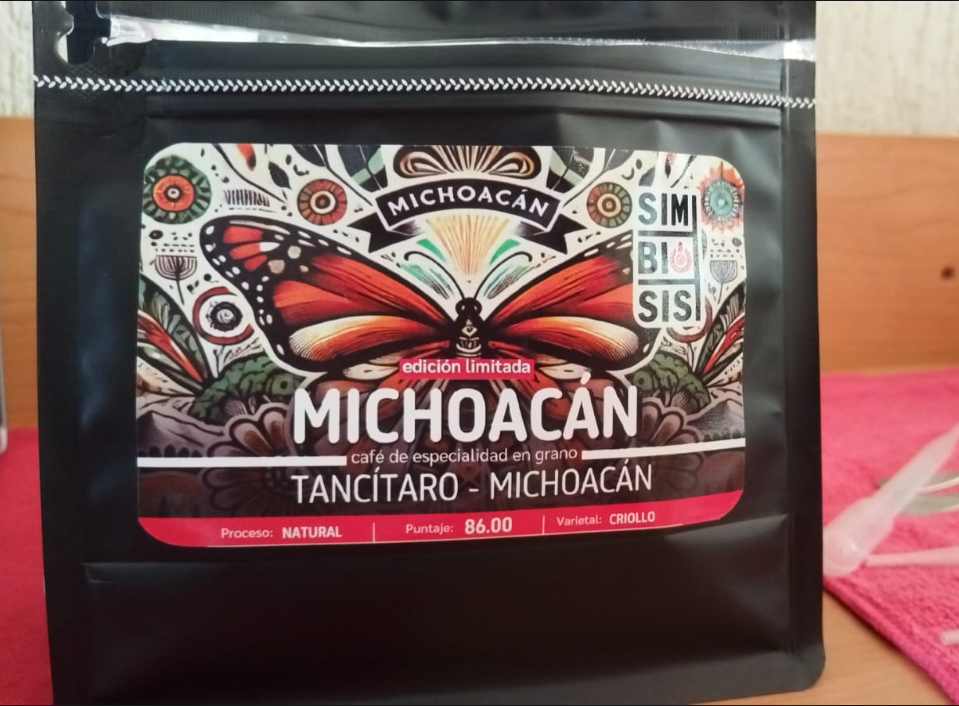
\includegraphics[width=0.6\textwidth]{1.png} % ajusta el ancho según convenga
    \caption{Descripción clara y concisa de la figura.}
    \label{fig:mi_figura2}
\end{figure}

En la bolsa dice \underline{Café de especialidad en grano}

\begin{figure}[H]
    \centering
	    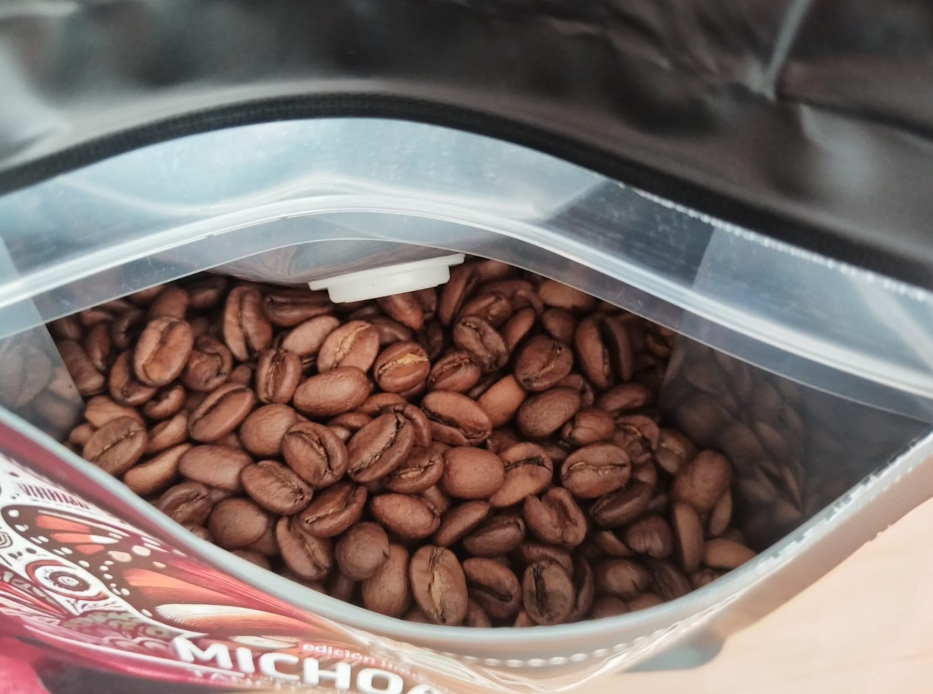
\includegraphics[width=0.6\textwidth]{2.png} % ajusta el ancho según convenga
    \caption{Descripción clara y concisa de la figura.}
    \label{fig:mi_figura2}
\end{figure}

\textbf{Orígen}: Michoacán (Tancítaro - Michoacán)

\textbf{Proceso}: Natural

\textbf{Puntaje}: 86.00

\textbf{Varietal}: Criollo

\textbf{Marca}: Simbiosis

\subsection{Gramajes}

Pesamos en la balanza los siguiente gramajes:

\begin{itemize}
\item[$\bullet$] 7.5\,g\\
\underline{Peso aproximado}: 7.5164\,g
\begin{figure}[H]
    \centering
	    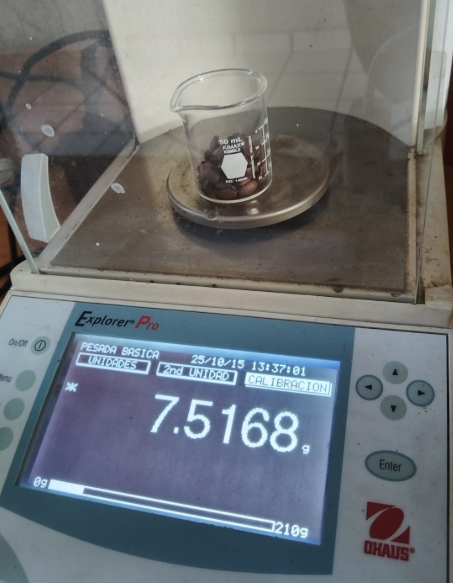
\includegraphics[width=0.4\textwidth]{3.png} % ajusta el ancho según convenga
    \caption{Descripción clara y concisa de la figura.}
    \label{fig:mi_figura2}
\end{figure}
\item[$\bullet$] 15\,g\\
\underline{Peso aproximado}: 14.9543\,g\\
\emph{Sabor}: Diluido, pero rico.
\begin{figure}[H]
    \centering
	    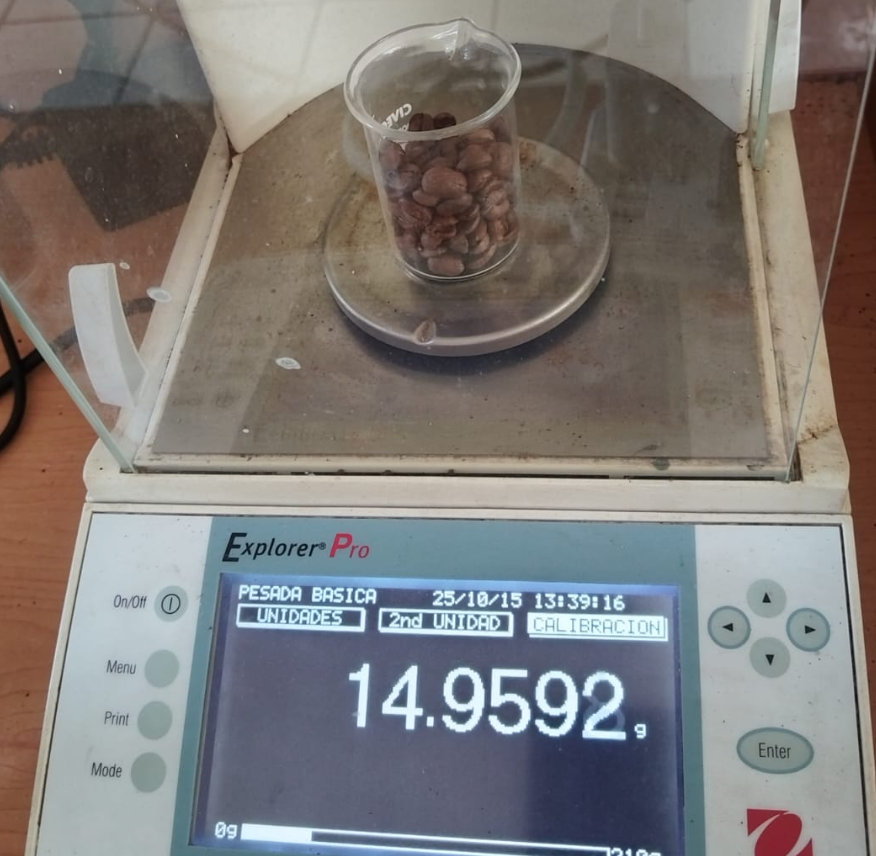
\includegraphics[width=0.4\textwidth]{4.png} % ajusta el ancho según convenga
    \caption{Descripción clara y concisa de la figura.}
    \label{fig:mi_figura2}
\end{figure}
\item[$\bullet$] 18\,g\\
\underline{Peso aproximado}: 18.02\,g
\begin{figure}[H]
    \centering
	    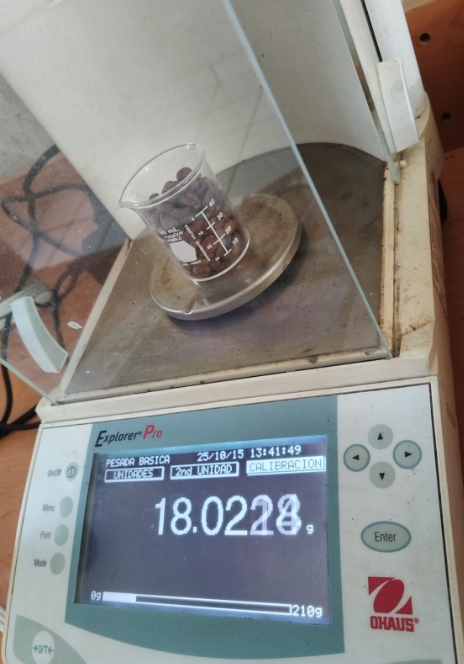
\includegraphics[width=0.4\textwidth]{5.png} % ajusta el ancho según convenga
    \caption{Descripción clara y concisa de la figura.}
    \label{fig:mi_figura2}
\end{figure}
\item[$\bullet$] 22.5\,g\\
\underline{Peso aproximado}: 22.5563\,g
\begin{figure}[H]
    \centering
	    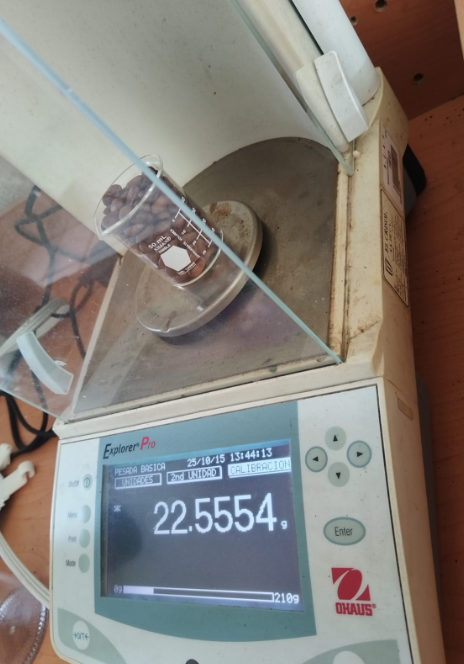
\includegraphics[width=0.4\textwidth]{6.png} % ajusta el ancho según convenga
    \caption{Descripción clara y concisa de la figura.}
    \label{fig:mi_figura2}
\end{figure}
\end{itemize}

En el molido ponemos las muelas en el nivel u opción 25, una molienda más gruesa.

\begin{figure}[H]
    \centering
	    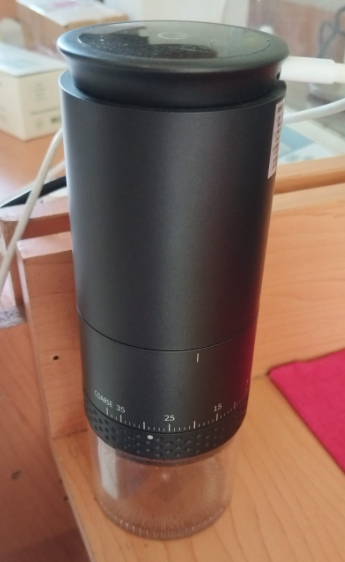
\includegraphics[width=0.4\textwidth]{7.png} % ajusta el ancho según convenga
    \caption{Descripción clara y concisa de la figura.}
    \label{fig:mi_figura2}
\end{figure}

\begin{figure}[H]
    \centering
	    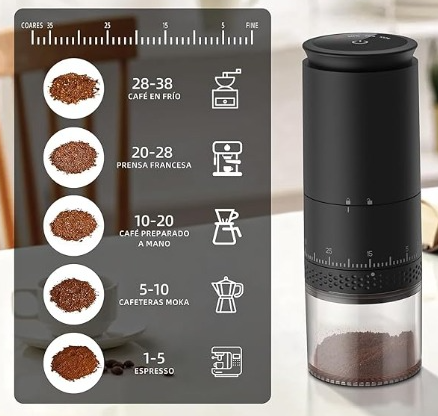
\includegraphics[width=0.4\textwidth]{8.png} % ajusta el ancho según convenga
    \caption{Descripción clara y concisa de la figura.}
    \label{fig:mi_figura2}
\end{figure}

\subsection{Resultados de las extracciones}

\subsubsection{Molienda}

\begin{figure}[H]
    \centering
	    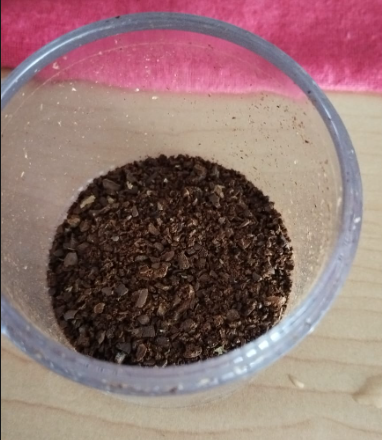
\includegraphics[width=0.4\textwidth]{9.png} % ajusta el ancho según convenga
    \caption{Descripción clara y concisa de la figura.}
    \label{fig:mi_figura2}
\end{figure}

Se ve una molienda algo gruesa, adecuada para prensa francesa.

\subsubsection{7.5\,g}

\begin{figure}[H]
    \centering
	    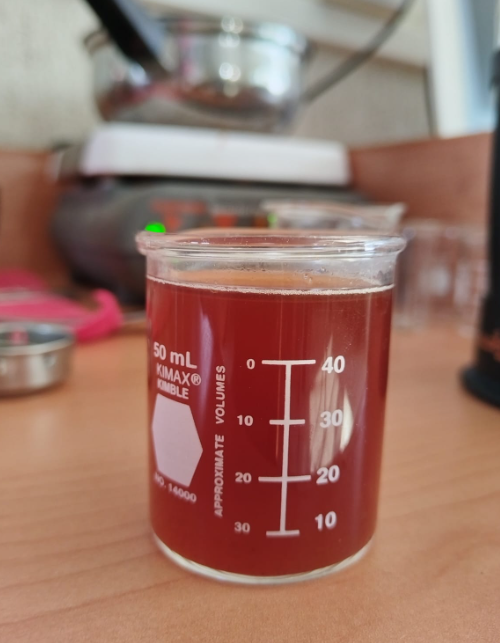
\includegraphics[width=0.4\textwidth]{10.png} % ajusta el ancho según convenga
    \caption{Descripción clara y concisa de la figura.}
    \label{fig:mi_figura2}
\end{figure}

\subsubsection{15\,g}

\begin{figure}[H]
    \centering
	    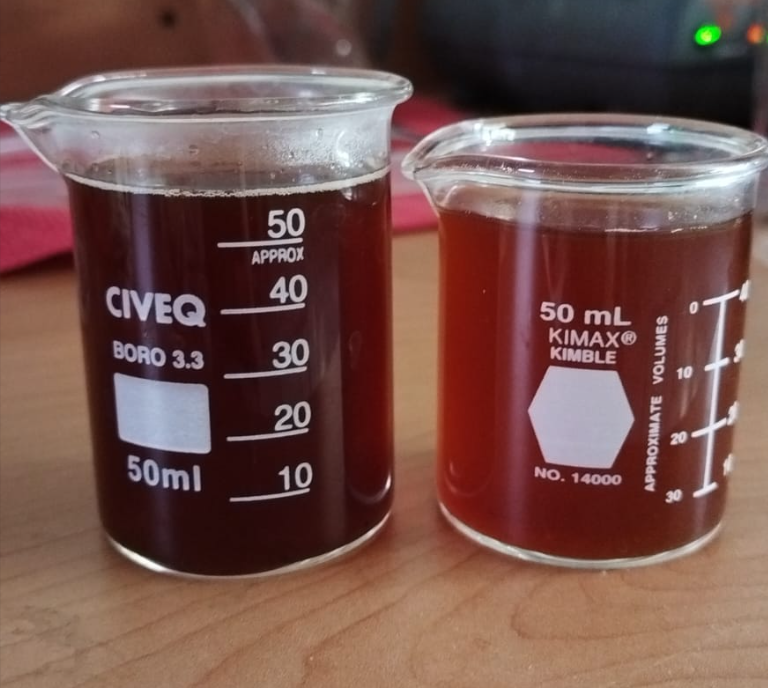
\includegraphics[width=0.4\textwidth]{11.png} % ajusta el ancho según convenga
    \caption{Descripción clara y concisa de la figura.}
    \label{fig:mi_figura2}
\end{figure}

\subsubsection{18\,g}

\begin{figure}[H]
    \centering
	    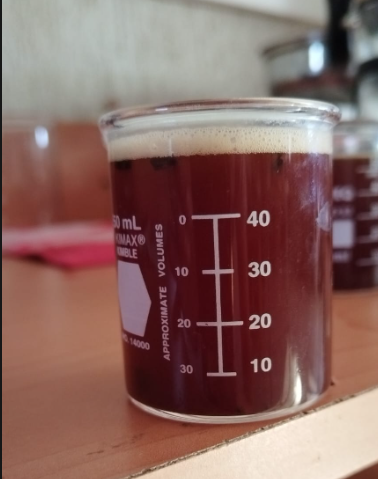
\includegraphics[width=0.4\textwidth]{12.png} % ajusta el ancho según convenga
    \caption{Descripción clara y concisa de la figura.}
    \label{fig:mi_figura2}
\end{figure}

\subsubsection{22.5\,g}

\begin{figure}[H]
    \centering
	    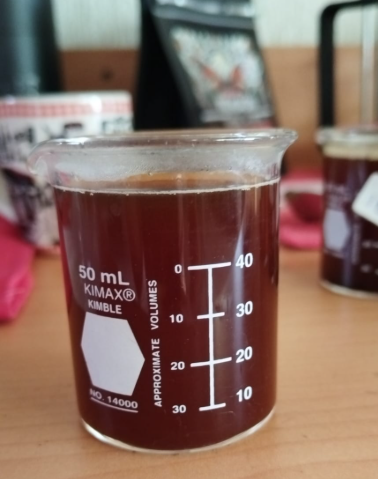
\includegraphics[width=0.4\textwidth]{13.png} % ajusta el ancho según convenga
    \caption{Descripción clara y concisa de la figura.}
    \label{fig:mi_figura2}
\end{figure}

Se elaboraron 2 pastilas de xMh y dos pastillas de RMh para michoacán

\section{Extracción Café de especialidad  - Espíritu café (Fecha: 16/10/2025)}

Este café tiene la siguiente ficha técnica:

\begin{figure}[H]
    \centering
	    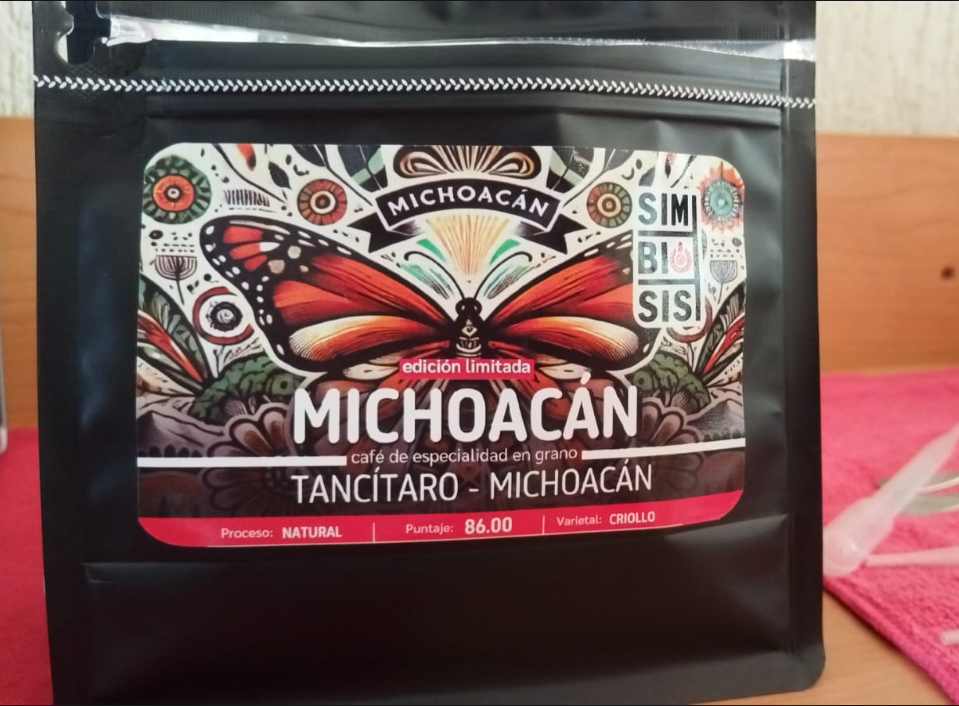
\includegraphics[width=0.6\textwidth]{1.png} % ajusta el ancho según convenga
    \caption{Descripción clara y concisa de la figura.}
    \label{fig:mi_figura2}
\end{figure}

En la bolsa dice \underline{Café de especialidad en grano}

\begin{figure}[H]
    \centering
	    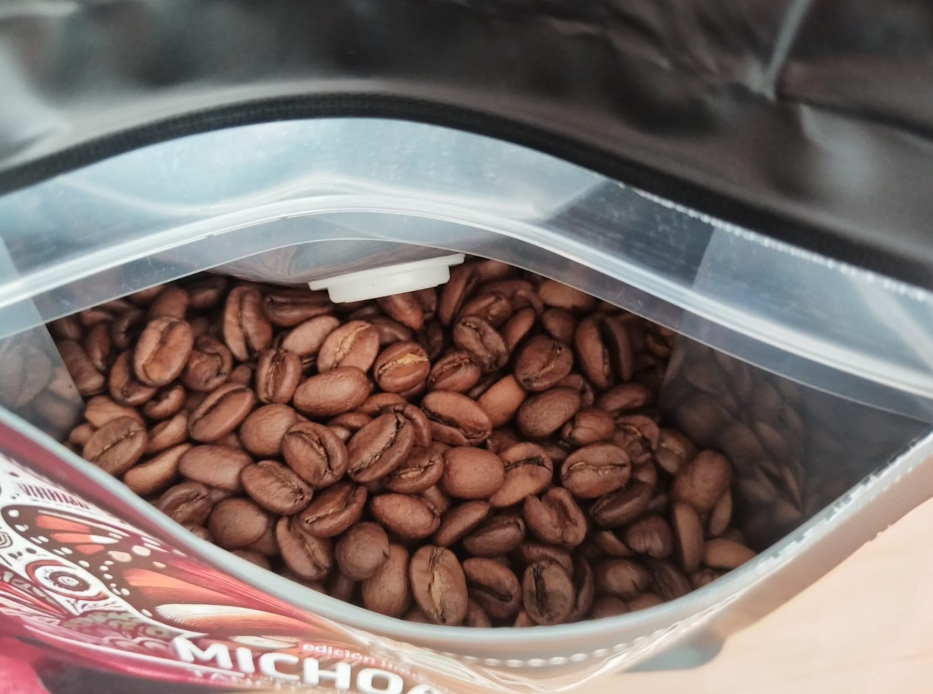
\includegraphics[width=0.6\textwidth]{2.png} % ajusta el ancho según convenga
    \caption{Descripción clara y concisa de la figura.}
    \label{fig:mi_figura2}
\end{figure}

\textbf{Orígen}: Michoacán (Tancítaro - Michoacán)

\textbf{Proceso}: Natural

\textbf{Puntaje}: 86.00

\textbf{Varietal}: Criollo

\textbf{Marca}: Simbiosis

EN aroma es muy rico, huele muy bien el de espiritu café. Ya viene molido, la moliendo no es tan gruesa, pero tampoco es tan fina. Adecuada para prensa francesa.

\subsection{Gramajes}

Pesamos en la balanza los siguiente gramajes:

\begin{itemize}
\item[$\bullet$] 7.5\,g\\
\underline{Peso aproximado}: 7.4950\,g
\begin{figure}[H]
    \centering
	    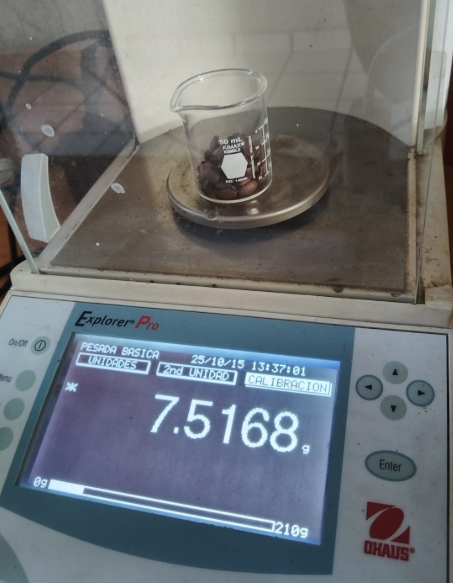
\includegraphics[width=0.4\textwidth]{3.png} % ajusta el ancho según convenga
    \caption{Descripción clara y concisa de la figura.}
    \label{fig:mi_figura2}
\end{figure}
\item[$\bullet$] 15\,g\\
\underline{Peso aproximado}: 15.0844\,g\\
\emph{Sabor}: Diluido, pero rico.
\begin{figure}[H]
    \centering
	    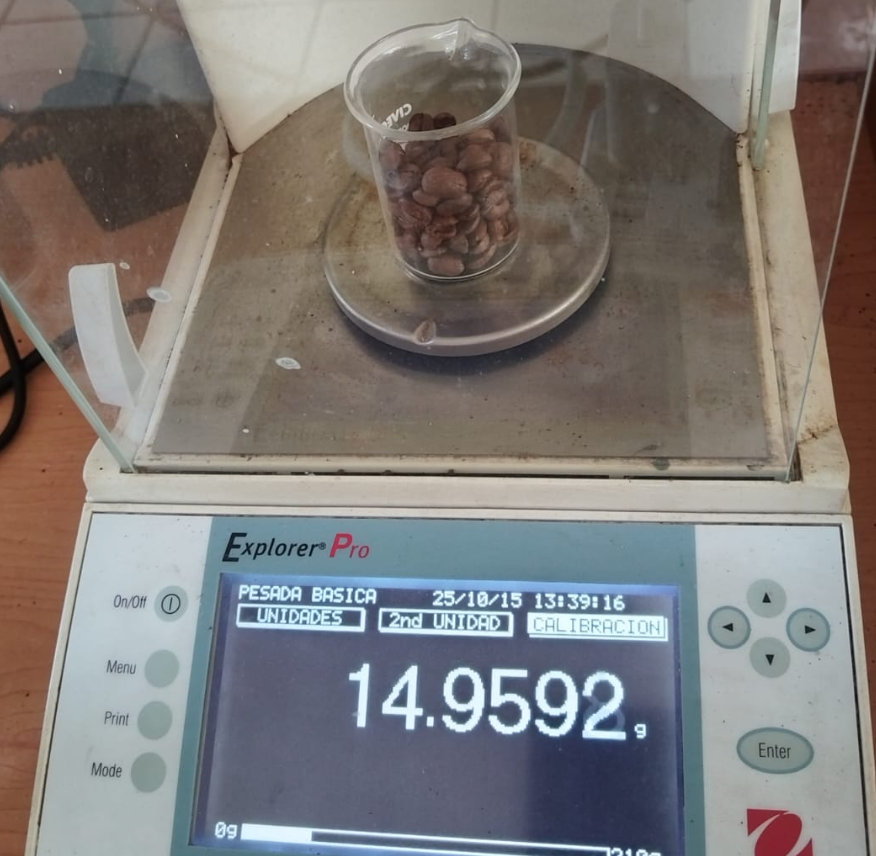
\includegraphics[width=0.4\textwidth]{4.png} % ajusta el ancho según convenga
    \caption{Descripción clara y concisa de la figura.}
    \label{fig:mi_figura2}
\end{figure}
\item[$\bullet$] 18\,g\\
\underline{Peso aproximado}: 18.0202\,g
\begin{figure}[H]
    \centering
	    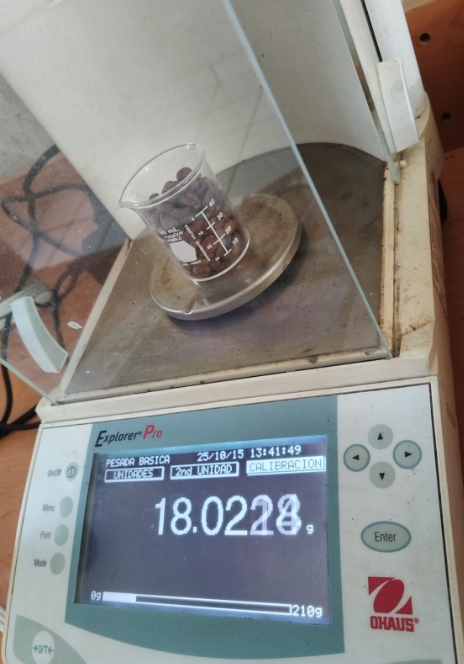
\includegraphics[width=0.4\textwidth]{5.png} % ajusta el ancho según convenga
    \caption{Descripción clara y concisa de la figura.}
    \label{fig:mi_figura2}
\end{figure}
\item[$\bullet$] 22.5\,g\\
\underline{Peso aproximado}: 22.4956\,g
\begin{figure}[H]
    \centering
	    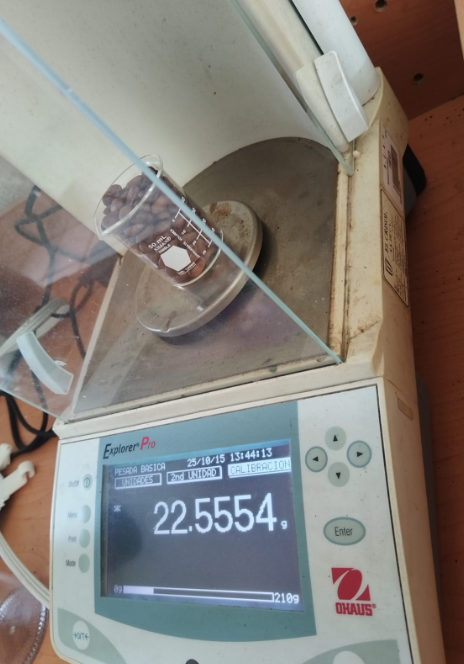
\includegraphics[width=0.4\textwidth]{6.png} % ajusta el ancho según convenga
    \caption{Descripción clara y concisa de la figura.}
    \label{fig:mi_figura2}
\end{figure}
\end{itemize}

En el molido ponemos las muelas en el nivel u opción 25, una molienda más gruesa.

\begin{figure}[H]
    \centering
	    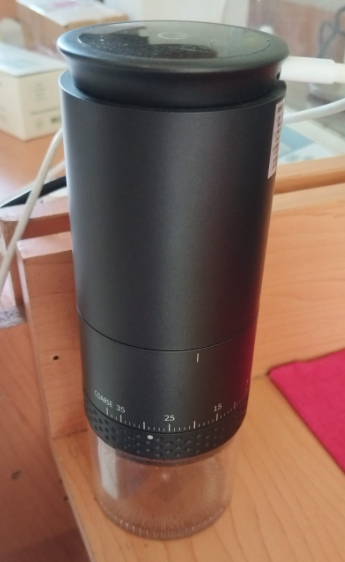
\includegraphics[width=0.4\textwidth]{7.png} % ajusta el ancho según convenga
    \caption{Descripción clara y concisa de la figura.}
    \label{fig:mi_figura2}
\end{figure}

\begin{figure}[H]
    \centering
	    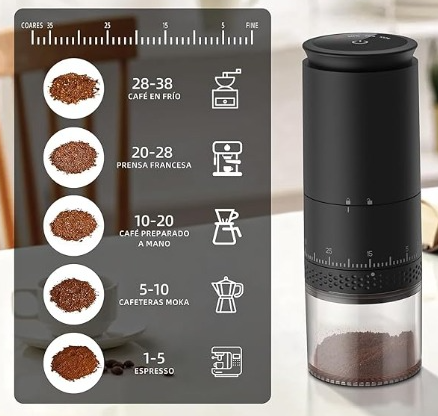
\includegraphics[width=0.4\textwidth]{8.png} % ajusta el ancho según convenga
    \caption{Descripción clara y concisa de la figura.}
    \label{fig:mi_figura2}
\end{figure}

\subsection{Resultados de las extracciones}

\subsubsection{Molienda}

\begin{figure}[H]
    \centering
	    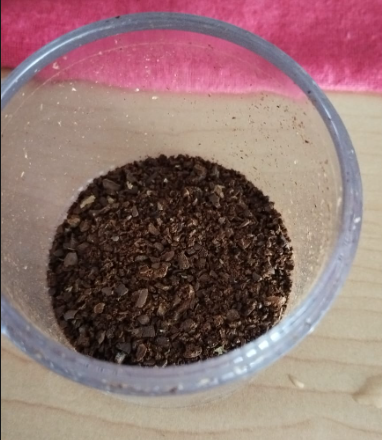
\includegraphics[width=0.4\textwidth]{9.png} % ajusta el ancho según convenga
    \caption{Descripción clara y concisa de la figura.}
    \label{fig:mi_figura2}
\end{figure}

Se ve una molienda algo gruesa, adecuada para prensa francesa.

\subsubsection{7.5\,g}

\begin{figure}[H]
    \centering
	    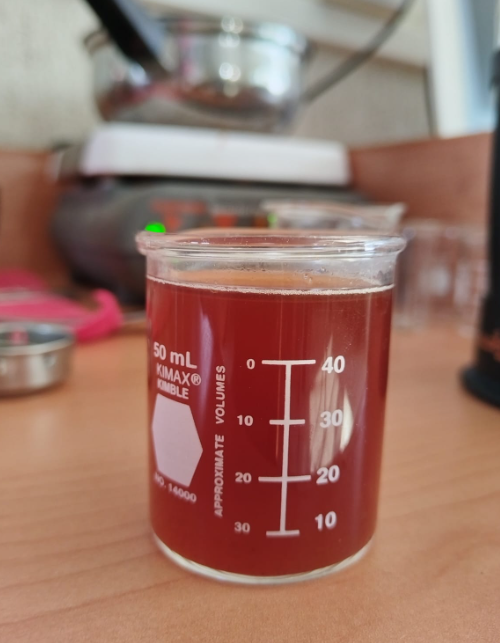
\includegraphics[width=0.4\textwidth]{10.png} % ajusta el ancho según convenga
    \caption{Descripción clara y concisa de la figura.}
    \label{fig:mi_figura2}
\end{figure}

\subsubsection{15\,g}

\begin{figure}[H]
    \centering
	    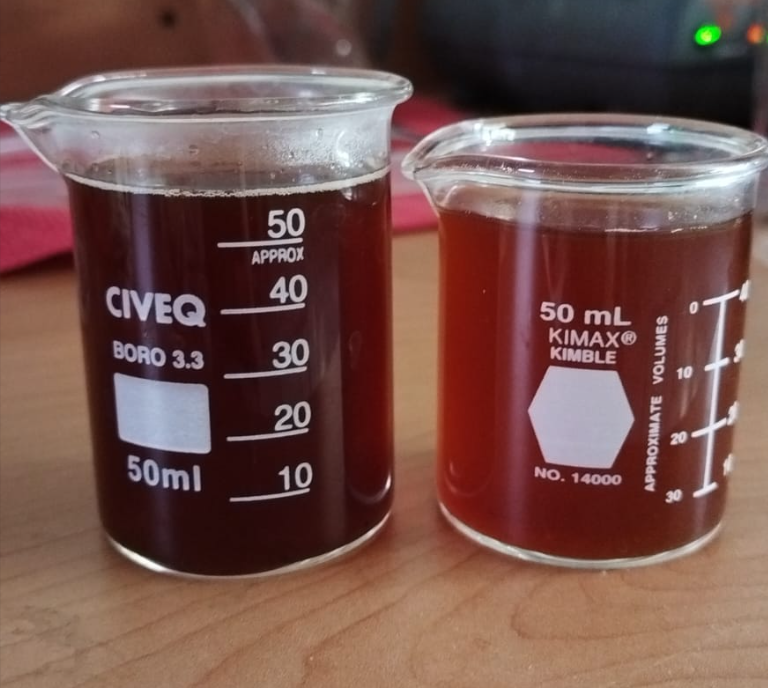
\includegraphics[width=0.4\textwidth]{11.png} % ajusta el ancho según convenga
    \caption{Descripción clara y concisa de la figura.}
    \label{fig:mi_figura2}
\end{figure}

\subsubsection{18\,g}

\begin{figure}[H]
    \centering
	    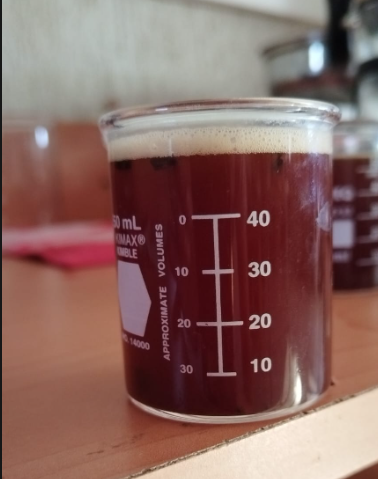
\includegraphics[width=0.4\textwidth]{12.png} % ajusta el ancho según convenga
    \caption{Descripción clara y concisa de la figura.}
    \label{fig:mi_figura2}
\end{figure}

\subsubsection{22.5\,g}

\begin{figure}[H]
    \centering
	    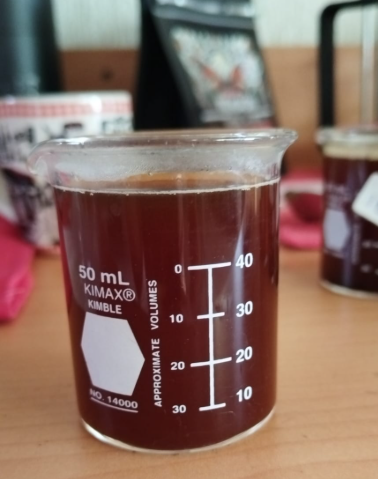
\includegraphics[width=0.4\textwidth]{13.png} % ajusta el ancho según convenga
    \caption{Descripción clara y concisa de la figura.}
    \label{fig:mi_figura2}
\end{figure}

Se elaboraron 2 pastilas de xMh y dos pastillas de RMh para michoacán
\end{document}
